\section{Magnetohydrodynamics in Astrophysics}
There are several phenomena in the universe that we can look at as magnetohydrodynamic in nature - planets consisting of metals, interplanetary space, but mainly - stars. If we talk about the nearest star - and the only one we are able to study well enough - the Sun - these phenomena include those that occur in the Sun's photosphere (the layer of Sun that is visible): Sun spots, but also phenomena that occur above the Sun (further from the center of the Sun): in Sun's chromosphere, or even corona (solar flares) - even phenomena that originate from the Sun, but then spread through our solar system - solar winds, space weather. All these phenomena have a large impact on the lives of all of us. For example solar flares (that are often followed by ejection of mass out of the Sun - the so called coronal mass ejections - CMEs) have impact on the Earth's magnetic field which in turn has impact on the electronic communication down on Earth (because the communication satellites used for transmissions may be damaged by the disturbances in the magnetic field). Also people operating at high altitudes, both in airplanes and manned space missions are exposed to the energetic particles coming from the Sun (this term is sometimes called \textit{cosmic rays}). For all the above reasons, it is of great importance to understand the phenomena of space weather, and other MHD phenomena that occur in space.

\subsection{Magnetic flux tube model of plasma}
We are interested in the process of evolution of the flux tube eruption. Such an eruption was captured during observations by \cite{miraClanek}, and the captured image is shown in \Cref{figure:observation} taken from \cite{miraClanek} (Figure 2 in the article).

\begin{figure}[H]
	\begin{center}
		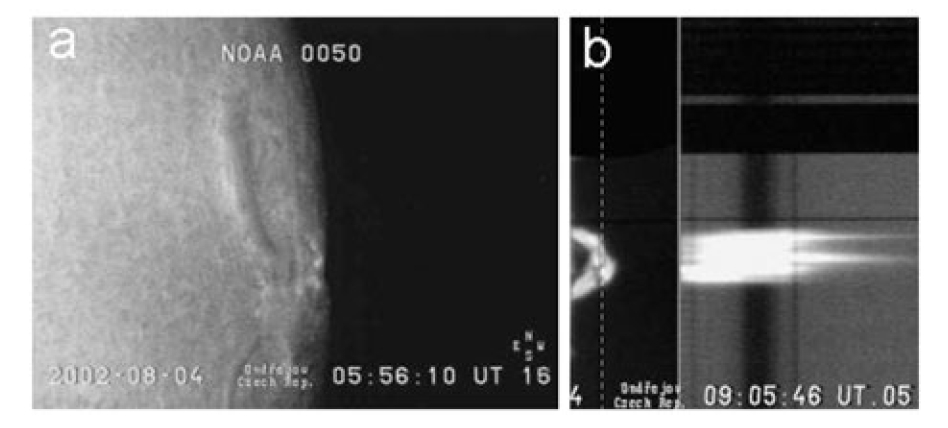
\includegraphics[width=0.5\textwidth]{img/td-setup/figure2fromHalpha.jpg}
	\caption{Observation of a limb event. $H\alpha$ slit-jaw is the middle (b) part, taken from \cite{miraClanek}.}
	\label{figure:observation}
	\end{center}
\end{figure}

For the modeling purposes, we are interested in the so-called $H\alpha$ slit-jaw which is the side-view of the magnetic flux tube during its evolution.
\paragraph{}
In order to model this phenomena physically, and geometrically, we utilize the magnetic field model by Titov and Demoulin (\cite{td}) which describes a twisted flux tube as part of a torus with minor radius $a$ (being the radius of the tube, not shown in \Cref{figure:td}) and major radius $R$ submerged below the photosphere of the Sun by $d < R$, oriented as in \Cref{figure:td} (taken from \cite{td}) with total current $I$.
\paragraph{}
The magnetic configuration is kept in a global equilibrium by the action of the Lorentz force due to the overlying magnetic field. The sources of this ambient field are modeled by a sub-photospheric line current $I_0$ and a pair of magnetic charges $+q, -q$ located at distance $L$ from the center of the torus, all located at the major axis of the torus.

\begin{figure}[H]
	\begin{center}
		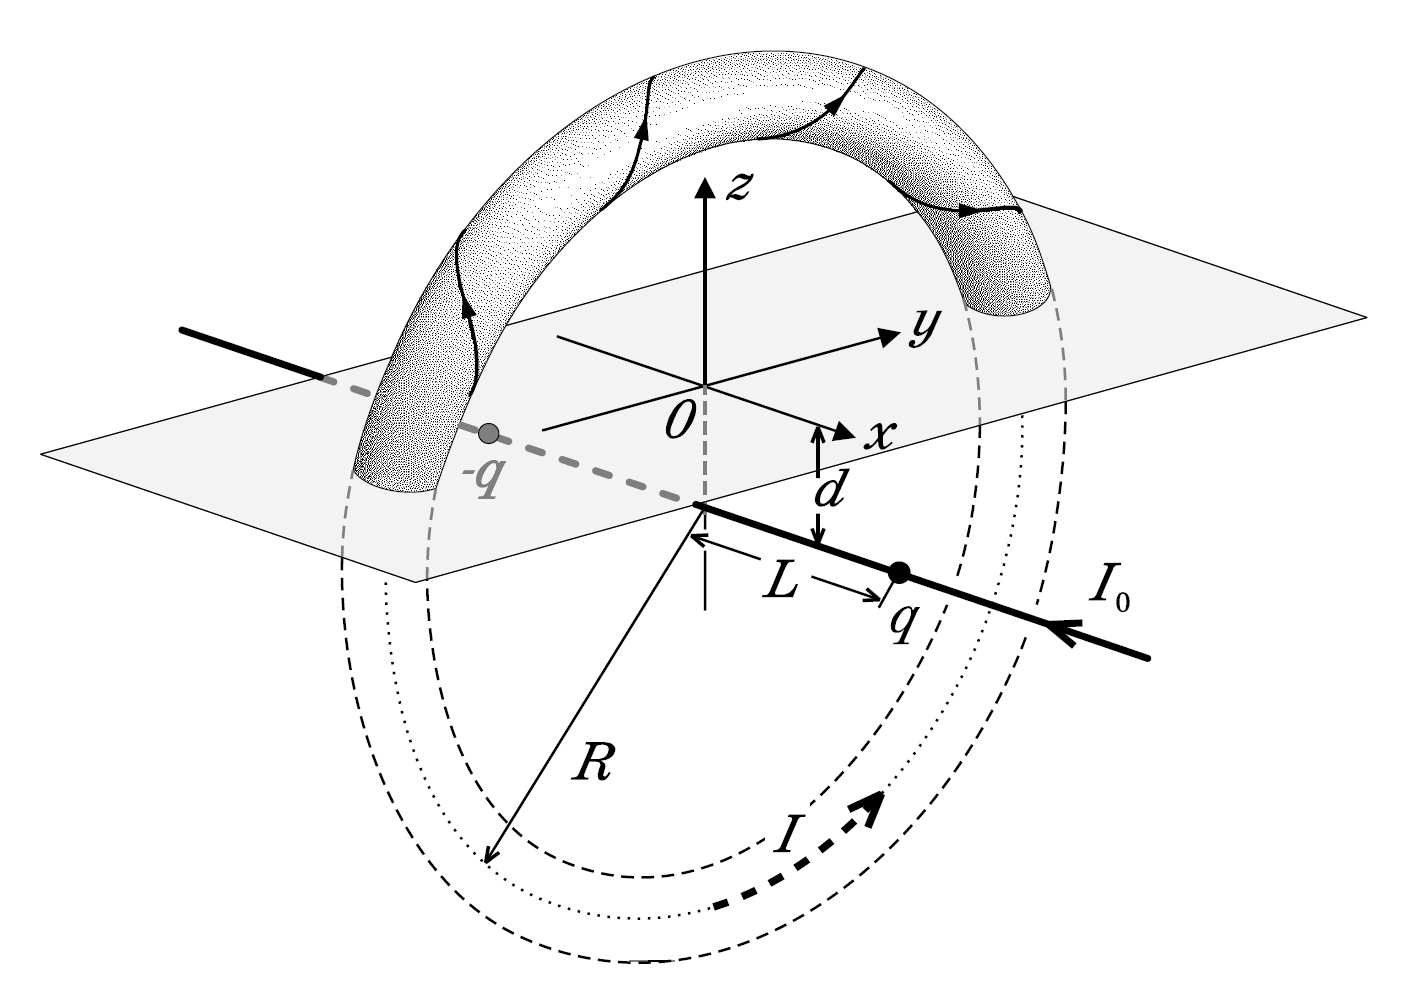
\includegraphics[width=0.5\textwidth]{img/td-setup/fromTD.jpg}
	\caption{The magnetic field under study, taken from \cite{td}.}
	\label{figure:td}
	\end{center}
\end{figure}

This geometrical/physical model needs to be properly modeled mathematically (including proper boundary conditions), then approached numerically, and finally computed using software that - in order to achieve reasonable accuracy of the solution - needs to be precisely implemented, must utilize approaches common in the high performance computing (HPC) field, and must be heavily optimized.
\paragraph{}
In the article \cite{miraClanek} which is a reference paper for this work, the model was set up according to observations, and numerical approach of Finite Difference Method (FDM) was used. The results obtained there are presented in \Cref{figure:miraResult0}, \Cref{figure:miraResult14}, and in order to compare them with \Cref{figure:observation}, also in the form in \Cref{figure:miraResultToCompare}.

\begin{figure}[H]
	\begin{center}
		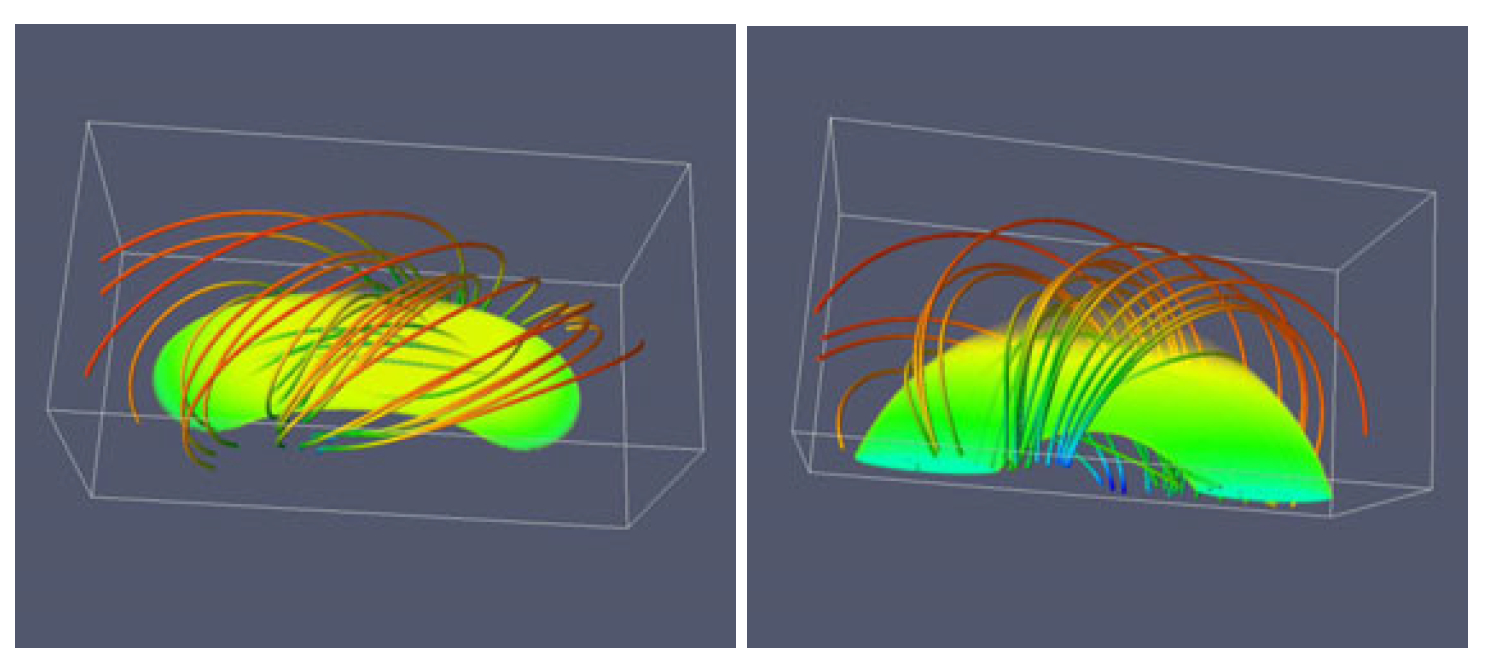
\includegraphics[width=0.5\textwidth]{img/td-setup/fromHalpha-initialFD.jpg}
	\caption{Results from \cite{miraClanek}, initial state, density volume and magnetic field isolines - top \& side view.}
	\label{figure:miraResult0}
	\end{center}
\end{figure}

\begin{figure}[H]
	\begin{center}
		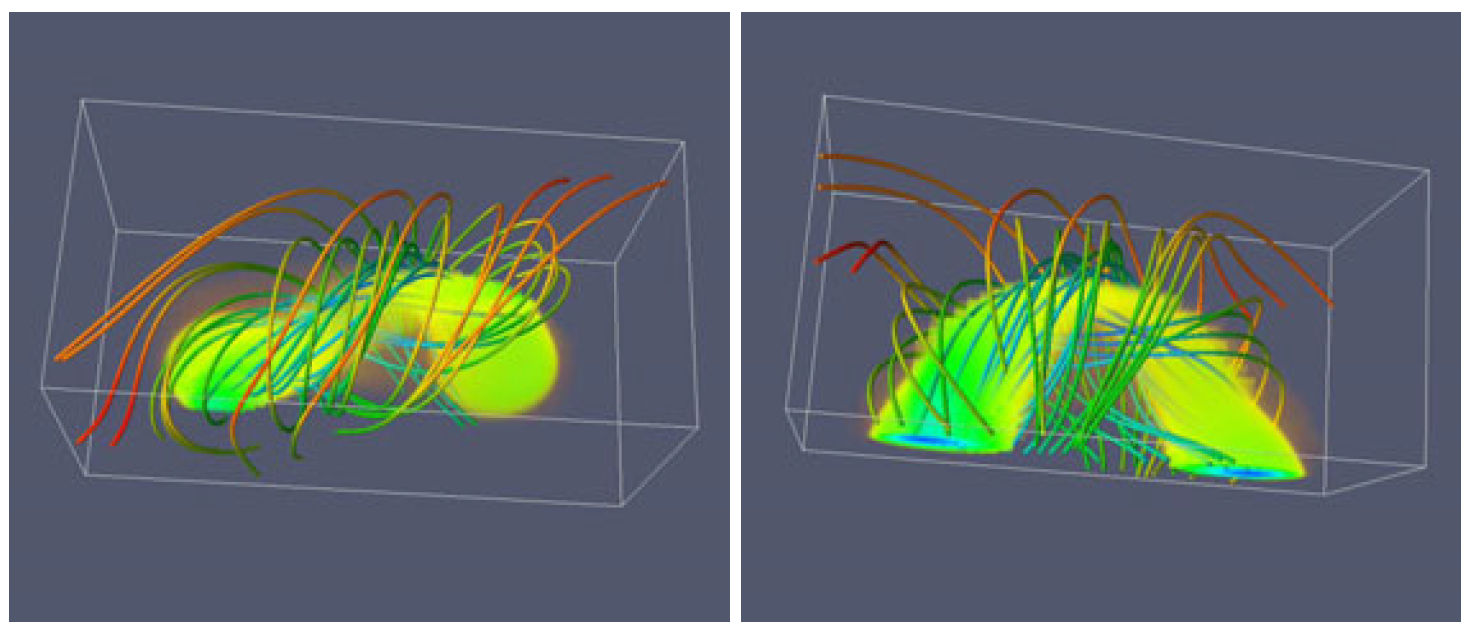
\includegraphics[width=0.5\textwidth]{img/td-setup/fromHalpha-14FD.jpg}
	\caption{Results from \cite{miraClanek}, state at $t = 14$, density volume and magnetic field isolines - top \& side view.}
	\label{figure:miraResult14}
	\end{center}
\end{figure}

\begin{figure}[H]
	\begin{center}
		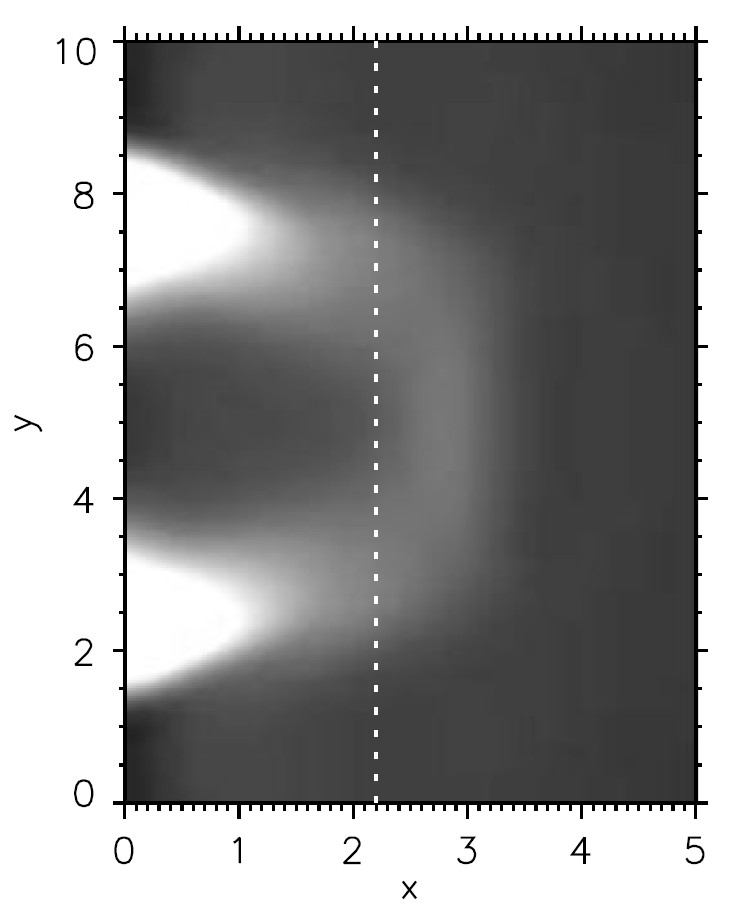
\includegraphics[width=0.5\textwidth]{img/td-setup/fromHalphaResult.jpg}
	\caption{Results from \cite{miraClanek}, time step chosen for best fit with \Cref{figure:observation}.}
	\label{figure:miraResultToCompare}
	\end{center}
\end{figure}

The aim of this work is to be able to compute results of such problems with much higher resolution, and more importantly to implement a generic solver which can handle any similar problem with arbitrary geometric and physical parameters.

\subsection{Magnetic reconnection}
An additional topic, interesting from the astrophysical point of view and related to magnetohydrodynamics, is the magnetic reconnection.
\paragraph{}
Magnetic reconnection occurs within electrically charged gases called plasmas. These charged particles interact strongly with the magnetic field, but at the same time their motions modify the magnetic field. Under normal conditions, the magnetic field lines inside plasmas don't break or merge with other field lines. But sometimes, as field lines get close to each other, the entire pattern changes and everything realign into a new configuration. The amount of energy released can be formidable. Magnetic reconnection taps into the stored energy of the magnetic field, converting it into heat and kinetic energy that sends particles streaming out along the field lines. Solar flares, which are among the phenomena which are the most important to study, are driven by magnetic reconnection - and thus studying magnetic reconnection is of great importance.
\paragraph{}
From the numerical perspective, to investigate such phenomena is to bring the complexity of multiple scales present in the physical world - magnetic reconnection occurs at substantially different scales than e.g. the solar flares. To handle this numerically with adequate resolution, and reasonable computational costs, the implementation must be able to limit the number of degrees of freedom used for the discretization to such that yield the largest accuracy increase - namely, in this work, this is achieved via a state-of-the-art Adaptive Mesh Refinement approach.